\documentclass[a4paper,12pt]{article}

\usepackage[utf8]{inputenc}
\usepackage[spanish]{babel}
\usepackage{amsmath, amssymb}
\usepackage{graphicx}
\usepackage{float}
\usepackage{booktabs}
\usepackage{xcolor}
\usepackage{listings}
\usepackage{caption}
\usepackage{fancyhdr}
\usepackage{hyperref}
\usepackage{tikz}
\usepackage{tabularx}
\usetikzlibrary{arrows.meta,positioning}

\hypersetup{
    colorlinks=true,
    linkcolor=blue,
    urlcolor=blue,
    pdftitle={Práctica 4 - MÁQUINA DE ESTADOS FINITOS (FSM)},
}

% === Definición de colores similares a Vivado ===
\definecolor{vivadoKeyword}{rgb}{0.6,0.0,0.6}
\definecolor{vivadoComment}{rgb}{0.0,0.5,0.0}
\definecolor{vivadoString}{rgb}{0.5,0.2,0.0}
\definecolor{vivadoBackground}{rgb}{0.97,0.97,0.97}

\lstdefinelanguage{VHDL}{
    morekeywords={library, use, entity, is, port, in, out, end, architecture, of, begin, signal, if, then, else, when, others, xor, and, or, not},
    sensitive=true,
    morecomment=[l]--,
    morestring=[b]",
}

\lstset{
    language=VHDL,
    backgroundcolor=\color{vivadoBackground},
    keywordstyle=\color{vivadoKeyword}\bfseries,
    commentstyle=\color{vivadoComment}\itshape,
    stringstyle=\color{vivadoString},
    basicstyle=\ttfamily\small,
    numbers=left,
    numberstyle=\tiny,
    numbersep=5pt,
    frame=single,
    breaklines=true,
    tabsize=2,
    captionpos=b
}

\title{Práctica N°4: Máquinas de Estados Finitos (FSM)}
\date{}

\begin{document}
\maketitle
\tableofcontents
\newpage

% =========================
% SECCIÓN: OBJETIVOS
% =========================
\section{Objetivos}

\subsection{Objetivo general}
Diseñar e implementar en \texttt{VHDL} un controlador de semáforo con visualización de cuenta regresiva en displays de 7 segmentos para la tarjeta Nexys A7-100T, que emplee una máquina de estados finitos (FSM) síncrona, multiplexado de displays y tratamiento robusto de entradas mediante \emph{debounce} y \emph{one-shot}.

\subsection{Objetivos específicos}
\begin{itemize}
    \item Modelar la lógica del semáforo como una FSM con estados y transiciones claramente definidas.
    \item Implementar divisores de reloj para generar un \emph{tick} de 1~Hz y una frecuencia de refresco adecuada para el multiplexado de 8 dígitos.
    \item Integrar un pulsador con sincronización a reloj, \emph{debounce} por tiempo y un pulso único (\emph{one-shot}) para accionar la reducción de tiempo o el salto de estado.
    \item Desarrollar un decodificador BCD a 7 segmentos \emph{activo en bajo} y una lógica de multiplexado estable para dos dígitos de conteo.
    \item Validar la coherencia de las salidas de LEDs por ejes (N/S, E/O) y la sincronía entre la visualización y la FSM.
\end{itemize}

\section{Marco Teórico.}

\subsection{Máquinas de estados}

Una máquina de estados finita (MEF), también conocida como autómata finito, es un modelo matemático utilizado para describir y representar sistemas que exhiben diferentes estados y transiciones entre ellos. Se utiliza en el campo de la computación y en la ingeniería para diseñar y analizar sistemas de control, protocolos de comunicación y lógica secuencial.

Una MEF consta de un conjunto finito de estados, donde cada estado representa una condición o configuración específica del sistema en un momento dado. Puede haber un estado inicial que representa el estado inicial del sistema y uno o más estados finales (o de aceptación) que indican que el sistema ha alcanzado un estado deseado o ha completado una secuencia de eventos.

\begin{figure}[H]
      \centering
      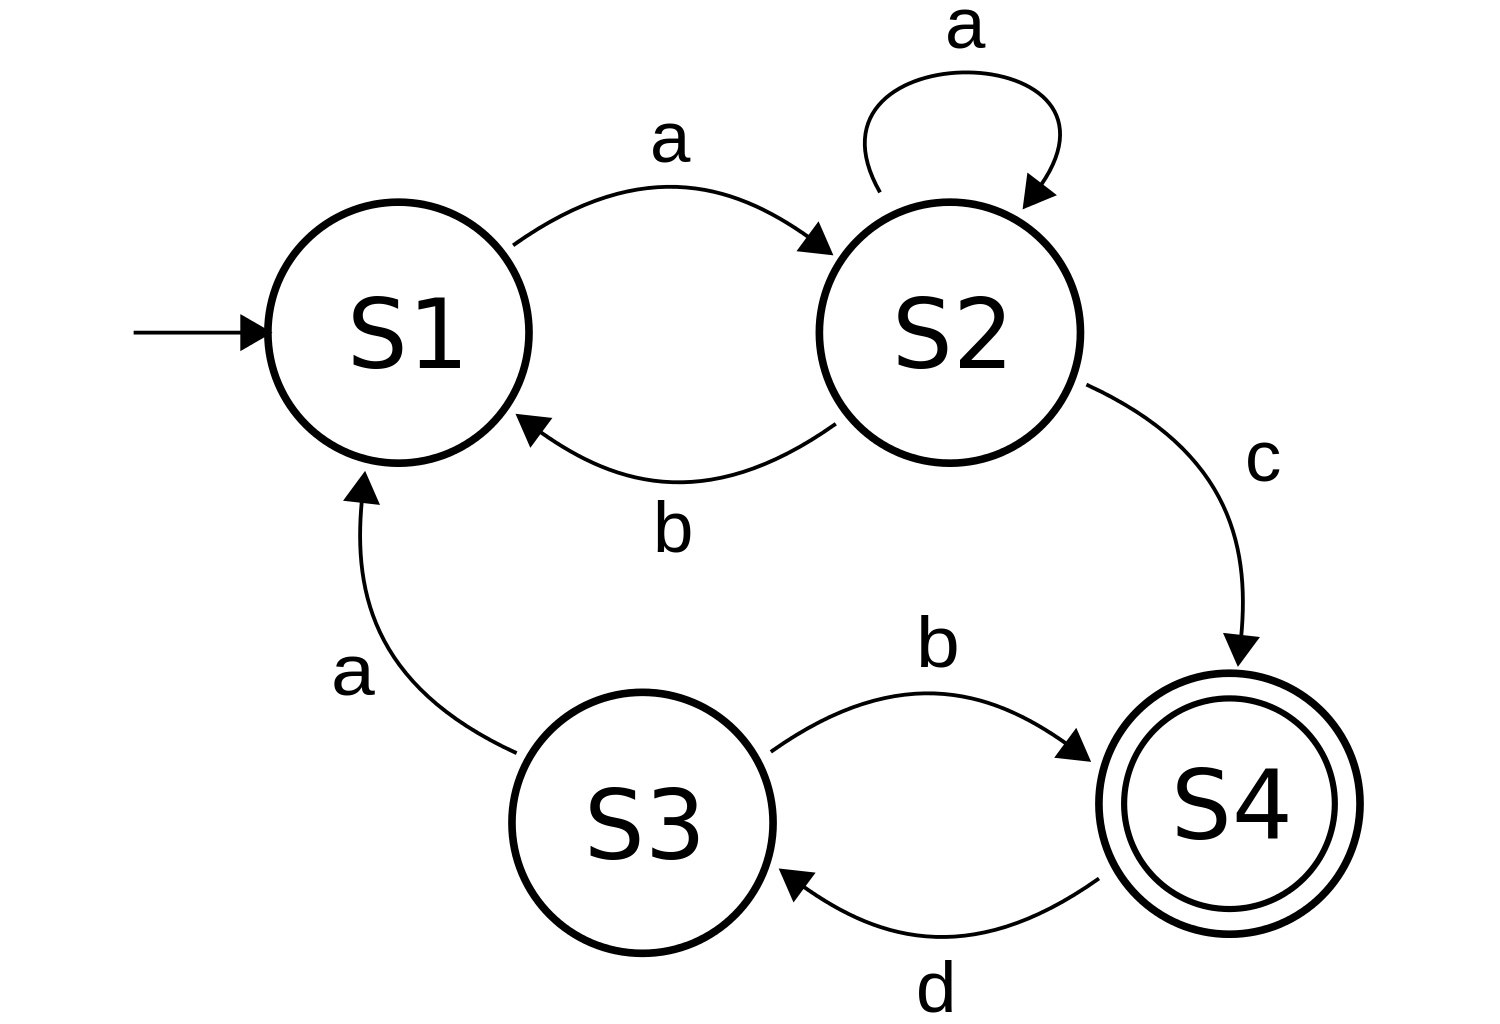
\includegraphics[width=0.5\textwidth]{maq est.png}
      \caption{Diagrama de una maquina de estados finitos} \label{fig}
  \end{figure}


Las Transiciones de un estado a otro se generan en respuesta a eventos de entrada externos e internos; a su vez estas transiciones y/o subsecuentes estados pueden generar otros eventos de salida. Se pueden representar mediante una tabla de transiciones, un diagrama de estados o mediante funciones de transición. \cite{alavi2016maquinas}

La implementación de una máquina de estados finita no es una técnica única, sino una variedad de métodos que comparten un principio común. En un nivel alto, existen dos formas de implementar una máquina de estados finita (se hablará de ellas más adelante). La primera opción implica el uso de una estructura if-else. Esta estrategia es fácil de entender e implementar, pero tiene desventajas significativas, el código se vuelve difícil de comprender ya que todo se agrupa en una única condición. 

El segundo método para implementar una MEF es utilizar una estructura switch. Esta permite escribir una función separada para cada estado y luego ejecutar una de estas funciones en función del estado actual. La ventaja de utilizar un switch es que facilita comprender el flujo de ejecución a través del código. Sin embargo, esta implementación no es muy escalable.

\subsubsection{Maquina de Moore}

Una máquina de Moore es un tipo de máquina  en la cual las salidas dependen únicamente del estado actual en el que se encuentra la máquina. Es decir, las salidas están asociadas directamente con los estados y no se ven influenciadas por las entradas del sistema.

En una máquina de Moore, cada estado tiene asociada una salida específica que se mantiene constante mientras la máquina se encuentre en ese estado. Cuando la máquina realiza una transición de estado, la salida puede cambiar según la nueva configuración. El cambio en las salidas ocurre únicamente cuando se produce una transición de estado y no está determinado por las entradas del sistema. \cite{alavimaquinas}
\begin{figure}[H]
      \centering
      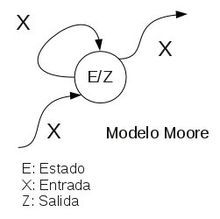
\includegraphics[width=0.5\textwidth]{moore.png}
      \caption{Diagrama de una maquina de Moore} \label{fig}
  \end{figure}


\subsubsection{Maquina de Mealy }

una Máquina de Mealy es un tipo de máquina de estados finitos que genera una salida basándose en su estado actual y una entrada. Esto significa que el Diagrama de estados incluirá ambas señales de entrada y salida para cada línea de transición.

En una máquina de Mealy, la salida puede cambiar instantáneamente cuando se produce una transición de estado y las entradas del sistema también cambian. Esto significa que las salidas pueden ser variables y dependen tanto del estado actual como de las entradas actuales. Por lo tanto, la respuesta del sistema en una máquina de Mealy puede ser más inmediata y sensible a los cambios en las entradas. \cite{de2003maquinas}

Las máquinas de Mealy se utilizan en aplicaciones donde las salidas deben ser sensibles a las entradas del sistema y el comportamiento del sistema puede cambiar rápidamente en función de los cambios en las entradas.

\begin{figure}[H]
      \centering
      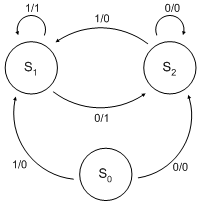
\includegraphics[width=0.5\textwidth]{mealy.png}
      \caption{Diagrama de una maquina de Mealy} \label{fig}
  \end{figure}

  \section{GPIO Externos en la Nexys A7-100T}

Una de las características más útiles de la tarjeta \textbf{Nexys A7-100T} es la presencia de conectores de propósito general (GPIO) accesibles para el usuario. Estos pines están agrupados en los encabezados denominados \textbf{Pmod Ports}, identificados como \textbf{JA, JB, JC y JD}. Cada uno de estos puertos permite conectar dispositivos externos tales como sensores, actuadores o módulos de comunicación.

\subsection{Distribución de los Pmod Ports}
Cada conector Pmod está compuesto por \textbf{8 señales de entrada/salida digitales}, organizadas en dos grupos de 4 pines. Además, cuentan con líneas de alimentación y tierra que permiten energizar dispositivos externos:

\begin{itemize}
    \item \textbf{8 pines GPIO}: programables desde el diseño en VHDL o Verilog.
    \item \textbf{2 pin de 3.3V fijo}: salida de tensión estable para alimentar periféricos externos.
    \item \textbf{2 pin de GND}: referencia común de tierra.
\end{itemize}

En total, cada puerto Pmod dispone de 12 pines (8 de propósito general, 2 de 3.3V, 2 de GND. Los niveles de tensión están limitados a \textbf{3.3V}, por lo que cualquier dispositivo conectado debe ser compatible con este estándar de lógica.

\subsection{Usos de los Pmod Ports}
Gracias a estos conectores, el estudiante puede extender las capacidades de la tarjeta de manera sencilla:
\begin{itemize}
    \item Conectar \textbf{módulos de sensores} (temperatura, luz, acelerómetros, etc.).
    \item Interconectar con \textbf{módulos de comunicación} (UART, SPI, I2C).
    \item Manejar \textbf{actuadores externos} (displays, relés, motores con driver).
\end{itemize}

De esta manera, la Nexys A7 se convierte en una plataforma flexible tanto para prácticas educativas como para prototipado de proyectos.

\subsection{Referencia Visual}
En la Figura~\ref{fig:pmod_ports} se muestra la disposición de los conectores Pmod JA, JB, JC y JD en la tarjeta, tomada del manual oficial de Digilent. Esto permitirá al estudiante identificar rápidamente qué puerto usar de acuerdo con el dispositivo externo que desee conectar.

\begin{figure}[H]
    \centering
    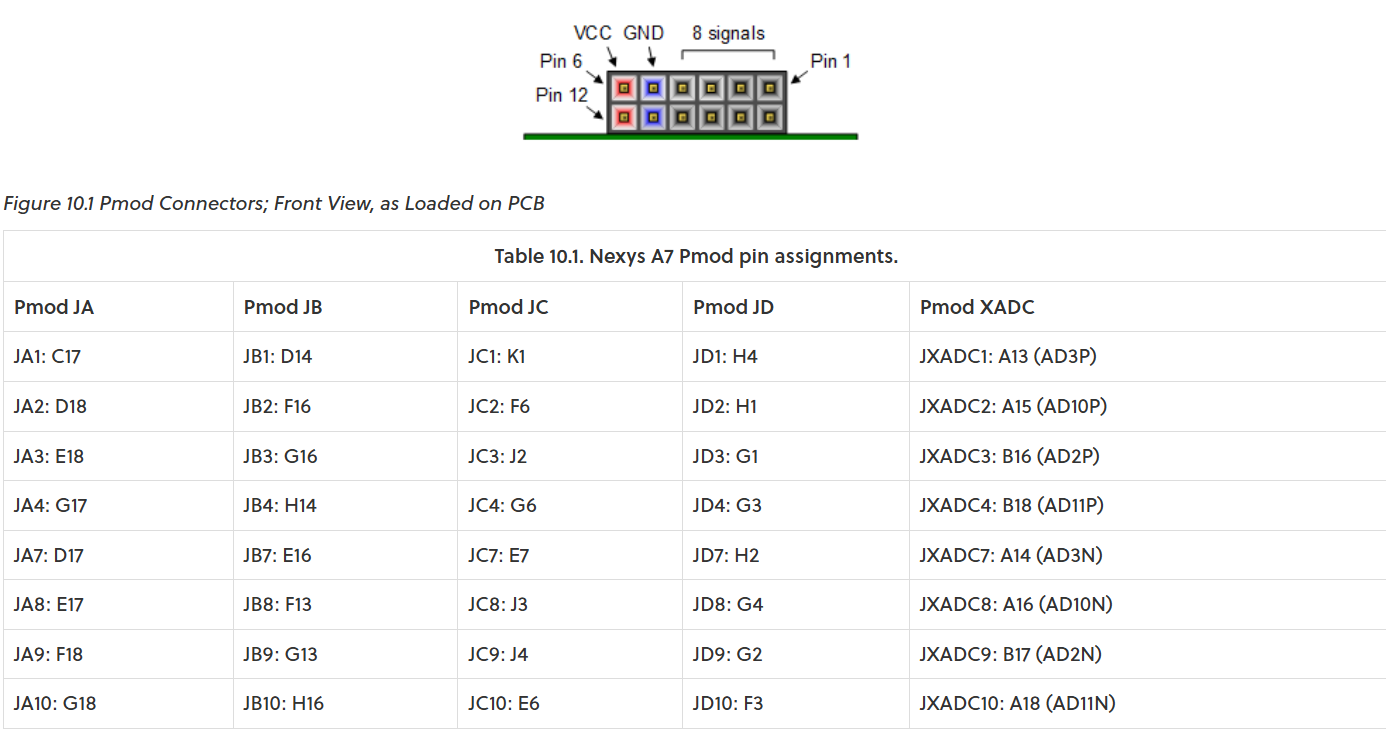
\includegraphics[width=0.7\textwidth]{pines.png}
    \caption{Conectores Pmod JA, JB, JC y JD de la Nexys A7-100T.}
    \label{fig:pmod_ports}
\end{figure}


% =========================
% SECCIÓN: DESCRIPCIÓN DEL CIRCUITO EN VHDL
% =========================
\newpage
\section{Descripción del circuito en VHDL}

\subsection*{Listado de código ()}
\begin{lstlisting}[language=VHDL, basicstyle=\ttfamily\footnotesize, numbers=left, numbersep=6pt, caption={Controlador de semáforo con cuenta regresiva y multiplexado de 7 segmentos.}, label={lst:semaforo}]
library IEEE;
use IEEE.STD_LOGIC_1164.ALL;
use IEEE.NUMERIC_STD.ALL;

entity semaforo_dia is
    Port (
        clk   : in  STD_LOGIC;                -- 100 MHz Nexys A7
        reset : in  STD_LOGIC;                -- Activo en alto
        btn_dec5 : in STD_LOGIC;              -- Boton: restar 5 s / saltar estado

        -- 7-seg multiplexados (activo en bajo)
        seg : out STD_LOGIC_VECTOR(0 to 6); -- CA..CG
        an  : out STD_LOGIC_VECTOR(7 downto 0); -- AN7..AN0 (activo en bajo)

        -- LEDs Norte
        led_n_rojo     : out STD_LOGIC;
        led_n_amarillo : out STD_LOGIC;
        led_n_verde    : out STD_LOGIC;

        -- LEDs Sur
        led_s_rojo     : out STD_LOGIC;
        led_s_amarillo : out STD_LOGIC;
        led_s_verde    : out STD_LOGIC;

        -- LEDs Este
        led_e_rojo     : out STD_LOGIC;
        led_e_amarillo : out STD_LOGIC;
        led_e_verde    : out STD_LOGIC;

        -- LEDs Oeste
        led_o_rojo     : out STD_LOGIC;
        led_o_amarillo : out STD_LOGIC;
        led_o_verde    : out STD_LOGIC
    );
end semaforo_dia;

architecture Behavioral of semaforo_dia is

    -- ======= FSM semaforo =======
    type state_type is (NS_VERDE, NS_AMARILLO, EO_VERDE, EO_AMARILLO);
    signal current_state, next_state : state_type := NS_VERDE;

    signal counter : integer range 0 to 10 := 10;

    -- ======= Relojes / divisores =======
    constant CLK_FREQ_HZ          : integer := 100_000_000;  -- Nexys A7
    -- Tick 1 Hz:
    constant ONE_HZ_DIV_MAX       : integer := CLK_FREQ_HZ - 1;
    signal one_hz_div             : integer range 0 to ONE_HZ_DIV_MAX := 0;
    signal tick_1s                : STD_LOGIC := '0';

    -- Multiplexado ~1 kHz por digito (8 digitos ? 8 kHz total)
    constant DIGITOS               : integer := 8;
    constant REFRESH_PER_DIGIT_HZ : integer := 1000;
    constant REFRESH_DIV_MAX      : integer := (CLK_FREQ_HZ / (REFRESH_PER_DIGIT_HZ * DIGITOS)) - 1; -- ~12500-1
    signal refresh_div            : integer range 0 to REFRESH_DIV_MAX := 0;
    signal mux_idx                : unsigned(2 downto 0) := (others => '0');  -- 0..7

    -- Buffer de digitos (0..9; 10=blank)
    type digit_array is array (0 to 7) of integer range 0 to 10;
    signal digits : digit_array := (others => 10); -- 10 = blanco

    -- ======= Decodificador 7-seg activo en bajo (CA..CG) =======
    -- OJO: valida que el orden de pines CA..CG de tu placa coincida con este mapa.
    function bcd_to_7seg_active_low(n: integer) return STD_LOGIC_VECTOR is
        -- 0=>"0000001" 1=>"1001111" 2=>"0010010" 3=>"0000110"
        -- 4=>"1001100" 5=>"0100100" 6=>"0100000" 7=>"0001111"
        -- 8=>"0000000" 9=>"0000100" blank=>"1111111"
        variable segs : STD_LOGIC_VECTOR(6 downto 0);
    begin
        case n is
            when 0  => segs := "0000001";
            when 1  => segs := "1001111";
            when 2  => segs := "0010010";
            when 3  => segs := "0000110";
            when 4  => segs := "1001100";
            when 5  => segs := "0100100";
            when 6  => segs := "0100000";
            when 7  => segs := "0001111";
            when 8  => segs := "0000000";
            when 9  => segs := "0000100";
            when others => segs := "1111111";
        end case;
        return segs;
    end function;

    -- ======= Sincronizacion / debounce / one-shot del boton =======
    constant DEBOUNCE_TICKS : integer := CLK_FREQ_HZ / 200; -- ~5 ms
    signal btn_sync0, btn_sync1 : STD_LOGIC := '0';
    signal btn_stable           : STD_LOGIC := '0';
    signal btn_stable_prev      : STD_LOGIC := '0';
    signal btn_pulse            : STD_LOGIC := '0';
    signal db_cnt               : integer range 0 to DEBOUNCE_TICKS := 0;

begin
    -- ======= Generador de tick 1 Hz =======
    process(clk)
    begin
        if rising_edge(clk) then
            if one_hz_div = ONE_HZ_DIV_MAX then
                one_hz_div <= 0;
                tick_1s    <= '1';
            else
                one_hz_div <= one_hz_div + 1;
                tick_1s    <= '0';
            end if;
        end if;
    end process;

    -- ======= Sincronizar boton a clk (2 FFs) =======
    process(clk)
    begin
        if rising_edge(clk) then
            btn_sync0 <= btn_dec5;
            btn_sync1 <= btn_sync0;
        end if;
    end process;

    -- ======= Debounce por tiempo =======
    process(clk)
    begin
        if rising_edge(clk) then
            if btn_sync1 = btn_stable then
                db_cnt <= 0; -- sin cambio
            else
                if db_cnt = DEBOUNCE_TICKS then
                    btn_stable <= btn_sync1; -- aceptar nuevo nivel
                    db_cnt <= 0;
                else
                    db_cnt <= db_cnt + 1;
                end if;
            end if;
        end if;
    end process;

    -- ======= One-shot en flanco ascendente del boton (despues del debounce) =======
    process(clk, reset)
    begin
        if reset = '1' then
            btn_stable_prev <= '0';
            btn_pulse       <= '0';
        elsif rising_edge(clk) then
            btn_pulse <= '0';
            if (btn_stable = '1') and (btn_stable_prev = '0') then
                btn_pulse <= '1';
            end if;
            btn_stable_prev <= btn_stable;
        end if;
    end process;

    -- ======= FSM + contador (prioridad al boton) =======
    process(clk, reset)
    begin
        if reset = '1' then
            current_state <= NS_VERDE;
            counter       <= 10;
        elsif rising_edge(clk) then
            -- 1) Boton: restar 5s o saltar estado si quedan <5s
            if btn_pulse = '1' then
                if counter >= 5 then
                    counter <= counter - 5;
                else
                    current_state <= next_state;
                    counter       <= 10;
                end if;

            -- 2) Tictac de 1 Hz
            elsif tick_1s = '1' then
                if counter > 0 then
                    counter <= counter - 1;
                else
                    current_state <= next_state;
                    counter       <= 10;
                end if;
            end if;
        end if;
    end process;

    -- ======= Siguiente estado =======
    process(current_state)
    begin
        case current_state is
            when NS_VERDE     => next_state <= NS_AMARILLO;
            when NS_AMARILLO  => next_state <= EO_VERDE;
            when EO_VERDE     => next_state <= EO_AMARILLO;
            when EO_AMARILLO  => next_state <= NS_VERDE;
        end case;
    end process;

    -- ======= LEDs segun estado (duplicados por eje) =======
    process(current_state)
        -- senales intermedias por eje
        variable ns_r, ns_y, ns_g : STD_LOGIC := '0';
        variable eo_r, eo_y, eo_g : STD_LOGIC := '0';
    begin
        -- por defecto apagado
        ns_r := '0'; ns_y := '0'; ns_g := '0';
        eo_r := '0'; eo_y := '0'; eo_g := '0';

        case current_state is
            when NS_VERDE =>
                ns_g := '1';     -- N/S verde
                eo_r := '1';     -- E/O rojo
            when NS_AMARILLO =>
                ns_y := '1';     -- N/S amarillo
                eo_r := '1';     -- E/O rojo
            when EO_VERDE =>
                eo_g := '1';     -- E/O verde
                ns_r := '1';     -- N/S rojo
            when EO_AMARILLO =>
                eo_y := '1';     -- E/O amarillo
                ns_r := '1';     -- N/S rojo
        end case;

        -- Duplicacion: N y S iguales; E y O iguales
        led_n_rojo     <= ns_r;  led_s_rojo     <= ns_r;
        led_n_amarillo <= ns_y;  led_s_amarillo <= ns_y;
        led_n_verde    <= ns_g;  led_s_verde    <= ns_g;

        led_e_rojo     <= eo_r;  led_o_rojo     <= eo_r;
        led_e_amarillo <= eo_y;  led_o_amarillo <= eo_y;
        led_e_verde    <= eo_g;  led_o_verde    <= eo_g;
    end process;

    -- ======= Calculo de digitos a mostrar (dos digitos, resto en blanco) =======
    process(counter)
        variable d, u : integer;
    begin
        d := counter / 10;
        u := counter mod 10;

        digits <= (others => 10); -- blanco
        digits(0) <= u;           -- AN0 = unidades
        digits(1) <= d;           -- AN1 = decenas
    end process;

    -- ======= Multiplexado de 8 digitos =======
    -- divisor de refresco
    process(clk)
    begin
        if rising_edge(clk) then
            if refresh_div = REFRESH_DIV_MAX then
                refresh_div <= 0;
                mux_idx     <= mux_idx + 1; -- 0..7
            else
                refresh_div <= refresh_div + 1;
            end if;
        end if;
    end process;

    -- seleccion de digito y anodos (activo en bajo)
    process(mux_idx, digits)
        variable an_v : STD_LOGIC_VECTOR(7 downto 0);
        variable seg_v: STD_LOGIC_VECTOR(6 downto 0);
        variable idx  : integer := to_integer(mux_idx);
    begin
        an_v := (others => '1');  -- todos apagados
        an_v(idx) := '0';         -- habilita uno (activo en bajo)

        seg_v := bcd_to_7seg_active_low(digits(idx));

        an  <= an_v;
        seg <= seg_v;
        -- dp eliminado
    end process;

end Behavioral;
\end{lstlisting}

% ===== Sub-secciones con fragmentos y explicación =====

% =======================
% Secciones didácticas por bloques (Semáforo día)
% Código antes de cada explicación
% =======================

\subsection{Entidad y puertos}

\begin{lstlisting}[language=VHDL, caption={Entidad y puertos del módulo}, label={lst:entidad-puertos}]
entity semaforo_dia is
  Port (
    clk        : in  STD_LOGIC;                -- 100 MHz Nexys A7
    reset      : in  STD_LOGIC;                -- Activo en alto
    btn_dec5   : in  STD_LOGIC;                -- Botón: restar 5 s / saltar estado

    -- 7-seg multiplexados (activo en bajo)
    seg        : out STD_LOGIC_VECTOR(0 to 6); -- CA..CG
    an         : out STD_LOGIC_VECTOR(7 downto 0); -- AN7..AN0 (activo en bajo)

    -- LEDs Norte
    led_n_rojo,     led_n_amarillo,     led_n_verde    : out STD_LOGIC;
    -- LEDs Sur
    led_s_rojo,     led_s_amarillo,     led_s_verde    : out STD_LOGIC;
    -- LEDs Este
    led_e_rojo,     led_e_amarillo,     led_e_verde    : out STD_LOGIC;
    -- LEDs Oeste
    led_o_rojo,     led_o_amarillo,     led_o_verde    : out STD_LOGIC
  );
end semaforo_dia;
\end{lstlisting}

\textbf{Idea clave.} Los displays y los ánodos son \emph{activos en bajo}, por lo que un ‘0’ enciende el segmento o el dígito. Los cuatro ejes (N, S, E, O) se controlan con salidas dedicadas, pero se agrupan en pares por eje (N/S y E/O) en la lógica interna.



\subsection{Tipos de datos y estados de la FSM}

\begin{lstlisting}[language=VHDL, caption={Tipos y registros de la máquina de estados}, label={lst:tipos-fsm}]
type state_type is (NS_VERDE, NS_AMARILLO, EO_VERDE, EO_AMARILLO);
signal current_state, next_state : state_type := NS_VERDE;

signal counter : integer range 0 to 10 := 10;
\end{lstlisting}

\textbf{Didáctica FSM.} Modelo de tipo \textbf{Moore}: las salidas (LEDs) dependen únicamente del \texttt{current\_state}. El ciclo es: \texttt{NS\_VERDE} $\rightarrow$ \texttt{NS\_AMARILLO} $\rightarrow$ \texttt{EO\_VERDE} $\rightarrow$ \texttt{EO\_AMARILLO} $\rightarrow$ \texttt{NS\_VERDE}.




\subsection{Divisores de reloj y generación de \texorpdfstring{$1$}{1}~Hz}

\begin{lstlisting}[language=VHDL, caption={Tick de 1 Hz y divisor de refresco para multiplexado}, label={lst:divisores}]
constant CLK_FREQ_HZ          : integer := 100_000_000;

-- Tick 1 Hz
constant ONE_HZ_DIV_MAX       : integer := CLK_FREQ_HZ - 1;
signal one_hz_div             : integer range 0 to ONE_HZ_DIV_MAX := 0;
signal tick_1s                : STD_LOGIC := '0';

process(clk)
begin
  if rising_edge(clk) then
    if one_hz_div = ONE_HZ_DIV_MAX then
      one_hz_div <= 0;
      tick_1s    <= '1';
    else
      one_hz_div <= one_hz_div + 1;
      tick_1s    <= '0';
    end if;
  end if;
end process;

-- Multiplexado ~1 kHz por dígito (8 dígitos -> ~8 kHz total)
constant DIGITOS               : integer := 8;
constant REFRESH_PER_DIGIT_HZ : integer := 1000;
constant REFRESH_DIV_MAX      : integer :=
  (CLK_FREQ_HZ / (REFRESH_PER_DIGIT_HZ * DIGITOS)) - 1;

signal refresh_div : integer range 0 to REFRESH_DIV_MAX := 0;
signal mux_idx     : unsigned(2 downto 0) := (others => '0');

process(clk)
begin
  if rising_edge(clk) then
    if refresh_div = REFRESH_DIV_MAX then
      refresh_div <= 0;
      mux_idx     <= mux_idx + 1;
    else
      refresh_div <= refresh_div + 1;
    end if;
  end if;
end process;
\end{lstlisting}

\textbf{Qué aprender.} El pulso \texttt{tick\_1s} (un ciclo por segundo) es la base del temporizador del semáforo. El índice \texttt{mux\_idx} recorre 0..7 para seleccionar cada dígito del display sin parpadeo visible.




\subsection{Sincronización, \emph{debounce} y \emph{one-shot} de \texttt{btn\_dec5}}

\begin{lstlisting}[language=VHDL, caption={Pipeline de entrada: sincronización, antirrebote y pulso único}, label={lst:debounce}]
-- Sincronización a 'clk'
process(clk)
begin
  if rising_edge(clk) then
    btn_sync0 <= btn_dec5;
    btn_sync1 <= btn_sync0;
  end if;
end process;

-- Debounce a ~5 ms
constant DEBOUNCE_TICKS : integer := CLK_FREQ_HZ / 200;
signal btn_stable, btn_stable_prev, btn_pulse : STD_LOGIC := '0';
signal db_cnt : integer range 0 to DEBOUNCE_TICKS := 0;

process(clk)
begin
  if rising_edge(clk) then
    if btn_sync1 = btn_stable then
      db_cnt <= 0;
    else
      if db_cnt = DEBOUNCE_TICKS then
        btn_stable <= btn_sync1;
        db_cnt <= 0;
      else
        db_cnt <= db_cnt + 1;
      end if;
    end if;
  end if;
end process;

-- One-shot
process(clk, reset)
begin
  if reset = '1' then
    btn_stable_prev <= '0';
    btn_pulse       <= '0';
  elsif rising_edge(clk) then
    btn_pulse <= '0';
    if (btn_stable = '1') and (btn_stable_prev = '0') then
      btn_pulse <= '1';
    end if;
    btn_stable_prev <= btn_stable;
  end if;
end process;
\end{lstlisting}

\textbf{Patrón universal.} Toda entrada asíncrona debe: (1) sincronizarse, (2) desrebotarse, (3) convertir flancos en pulsos de un ciclo. Esto evita metaestabilidad y múltiples disparos indeseados.


\subsection{Registro de estado y contador con prioridad al botón}

\begin{lstlisting}[language=VHDL, caption={Secuencial: prioridad al botón, luego al tick}, label={lst:estado-contador}]
process(clk, reset)
begin
  if reset = '1' then
    current_state <= NS_VERDE;
    counter       <= 10;

  elsif rising_edge(clk) then
    -- 1) Botón: restar 5s o saltar estado si quedan <5s
    if btn_pulse = '1' then
      if counter >= 5 then
        counter <= counter - 5;
      else
        current_state <= next_state;
        counter       <= 10;
      end if;

    -- 2) Tictac de 1 Hz
    elsif tick_1s = '1' then
      if counter > 0 then
        counter <= counter - 1;
      else
        current_state <= next_state;
        counter       <= 10;
      end if;
    end if;
  end if;
end process;
\end{lstlisting}

\textbf{Lección.} Este proceso es el \emph{registro de estado} canónico de una FSM: solo cambia en flancos de reloj o \texttt{reset}. La prioridad al botón define un comportamiento determinista cuando el usuario interactúa.

\newpage


\subsection{Lógica de transición (\texttt{next\_state})}

\begin{lstlisting}[language=VHDL, caption={Combinacional: cálculo de \texttt{next\_state}}, label={lst:next-state}]
process(current_state)
begin
  case current_state is
    when NS_VERDE     => next_state <= NS_AMARILLO;
    when NS_AMARILLO  => next_state <= EO_VERDE;
    when EO_VERDE     => next_state <= EO_AMARILLO;
    when EO_AMARILLO  => next_state <= NS_VERDE;
  end case;
end process;
\end{lstlisting}

\textbf{FSM en tres procesos.} Separar (1) registro de estado, (2) siguiente estado y (3) salidas simplifica verificación, síntesis y reutilización. El alumno debe adoptar este patrón como \emph{best practice}.


\subsection{Asignación de salidas (LEDs por eje)}

\begin{lstlisting}[language=VHDL, caption={Combinacional: salidas tipo Moore para LEDs}, label={lst:salidas-leds}]
process(current_state)
  variable ns_r, ns_y, ns_g : STD_LOGIC := '0';
  variable eo_r, eo_y, eo_g : STD_LOGIC := '0';
begin
  ns_r := '0'; ns_y := '0'; ns_g := '0';
  eo_r := '0'; eo_y := '0'; eo_g := '0';
  case current_state is
    when NS_VERDE     => ns_g := '1'; eo_r := '1';
    when NS_AMARILLO  => ns_y := '1'; eo_r := '1';
    when EO_VERDE     => eo_g := '1'; ns_r := '1';
    when EO_AMARILLO  => eo_y := '1'; ns_r := '1';
  end case;

  -- Duplicación por eje
  led_n_rojo     <= ns_r;  led_s_rojo     <= ns_r;
  led_n_amarillo <= ns_y;  led_s_amarillo <= ns_y;
  led_n_verde    <= ns_g;  led_s_verde    <= ns_g;

  led_e_rojo     <= eo_r;  led_o_rojo     <= eo_r;
  led_e_amarillo <= eo_y;  led_o_amarillo <= eo_y;
  led_e_verde    <= eo_g;  led_o_verde    <= eo_g;
end process;
\end{lstlisting}

\textbf{Claves.} Las salidas dependen solo del estado actual (Moore). La duplicación N/S y E/O garantiza consistencia física de los dos semáforos por eje.


\subsection{Decodificador BCD a 7 segmentos (activo en bajo)}

\begin{lstlisting}[language=VHDL, caption={Función BCD a 7-seg activo en bajo}, label={lst:decoder-7seg}]
function bcd_to_7seg_active_low(n: integer) return STD_LOGIC_VECTOR is
  -- 0=>"0000001" ... 9=>"0000100", blank=>"1111111"
  variable segs : STD_LOGIC_VECTOR(6 downto 0);
begin
  case n is
    when 0  => segs := "0000001";
    when 1  => segs := "1001111";
    when 2  => segs := "0010010";
    when 3  => segs := "0000110";
    when 4  => segs := "1001100";
    when 5  => segs := "0100100";
    when 6  => segs := "0100000";
    when 7  => segs := "0001111";
    when 8  => segs := "0000000";
    when 9  => segs := "0000100";
    when others => segs := "1111111";
  end case;
  return segs;
end function;
\end{lstlisting}

\textbf{Nota.} Verifica el mapeo \texttt{CA..CG} de tu placa: si el orden físico difiere, ajusta los bits del patrón. Mantén el convenio \texttt{(6 downto 0)} también en el puerto \texttt{seg} para coherencia.

\newpage


\subsection{Cálculo de dígitos (decenas y unidades)}

\begin{lstlisting}[language=VHDL, caption={Buffer de dígitos y partición decenas/unidades}, label={lst:buffer-digitos}]
type digit_array is array (0 to 7) of integer range 0 to 10;
signal digits : digit_array := (others => 10); -- 10 = blanco

process(counter)
  variable d, u : integer;
begin
  d := counter / 10;
  u := counter mod 10;

  digits <= (others => 10); -- blanco
  digits(0) <= u;           -- AN0 = unidades
  digits(1) <= d;           -- AN1 = decenas
end process;
\end{lstlisting}

\textbf{Buena práctica.} Los dígitos no usados quedan en “blanco” (1111111). Si deseas compatibilidad con 4 dígitos, reserva índices y añade símbolos (p.ej., guion cuando \texttt{counter} sea negativo en otras prácticas).


\subsection{Multiplexado de 8 dígitos}

\begin{lstlisting}[language=VHDL, caption={Selección de dígito y actualización de ánodos/segmentos}, label={lst:mux-digitos}]
process(mux_idx, digits)
  variable an_v : STD_LOGIC_VECTOR(7 downto 0);
  variable seg_v: STD_LOGIC_VECTOR(6 downto 0);
  variable idx  : integer := to_integer(mux_idx);
begin
  an_v := (others => '1');   -- todos apagados (activo en bajo)
  an_v(idx) := '0';          -- habilita uno

  seg_v := bcd_to_7seg_active_low(digits(idx));

  an  <= an_v;
  seg <= seg_v;
end process;
\end{lstlisting}

\textbf{Concepto.} \texttt{mux\_idx} selecciona el dígito activo y el decodificador determina el patrón de segmentos. La frecuencia efectiva es suficientemente alta para eliminar parpadeo.




% =======================
% Enfoque final: patrón universal de FSM
% =======================
\subsection{Patrón universal para cualquier máquina de estados}

\noindent Para diseñar \textbf{cualquier} FSM en VHDL, sigue este esqueleto de tres procesos:
\begin{enumerate}
  \item \textbf{Registro de estado} (\emph{secuencial}): actualiza \texttt{current\_state} en flanco de reloj y gestiona \texttt{reset}.
  \item \textbf{Próximo estado} (\emph{combinacional}): calcula \texttt{next\_state} a partir de \texttt{current\_state} y entradas sincronizadas.
  \item \textbf{Salidas} (\emph{combinacional}): define señales de salida solo en función del estado (Moore) o del estado y entradas (Mealy).
\end{enumerate}

\noindent Este patrón, junto con el pipeline de entradas (sincronización + debounce + one-shot) y una temporización basada en ticks, permite construir FSMs robustas y escalables para cualquier problema de control digital.



% =========================
% SECCIÓN: DIAGRAMA DE BLOQUES
% =========================
\subsection{Diagrama de bloques}
\begin{figure}[H]
    \centering
    % Reemplaza 'bloques_semaforo.png' por tu imagen real
    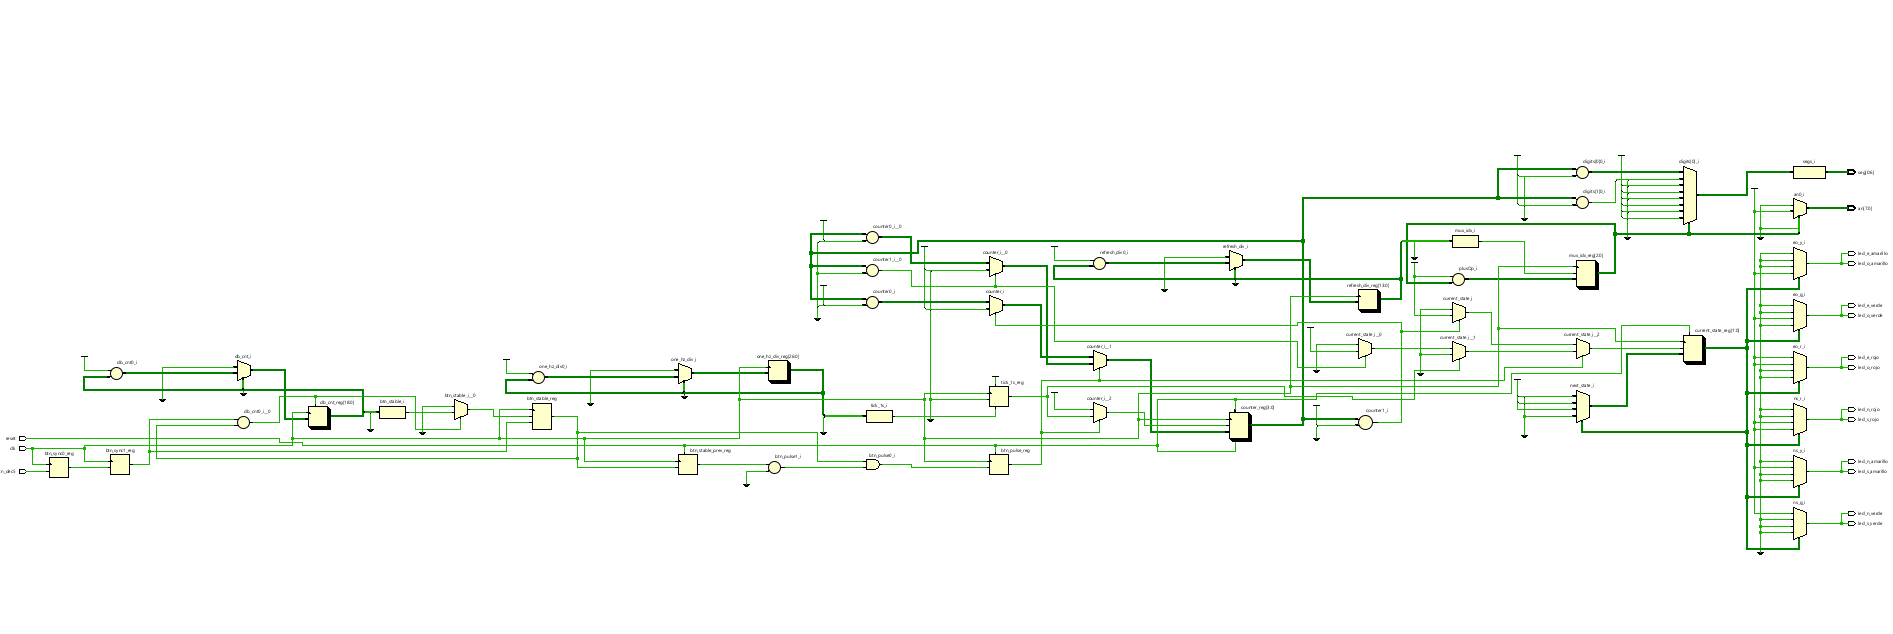
\includegraphics[width=0.95\linewidth]{Esquematicos/esquema.png}
    \caption{Diagrama de bloques: divisores de reloj, tratamiento de botón, FSM, lógica de salidas y subsistema de visualización (decodificador + multiplexado).}
    \label{fig:bloques-semaforo}
\end{figure}

% =======================
% Subsección: Mapeo de pines y niveles eléctricos
% =======================

\subsection{Mapeo de pines y niveles eléctricos (Nexys A7)}

En esta subsección se presenta el \textbf{mapeo lógico–físico} de todas las señales del diseño hacia pines del FPGA. Las tablas están organizadas por función: control/temporización, displays de 7 segmentos y salidas a LEDs por eje. Todas las E/S usan \texttt{LVCMOS33}.

\paragraph{Convenciones clave.}
\begin{itemize}
  \item Los ánodos del display (\texttt{an[7:0]}) y los segmentos (\texttt{seg[6:0]}) son \textbf{activos en bajo}.
  \item Para mantener coherencia con el decodificador, adopta la convención \textbf{\texttt{seg(6\,downto\,0)}} $\equiv$ \texttt{CA..CG}. Si tu entidad declara \texttt{seg(0 to 6)}, homogeneiza direcciones o ajusta el orden de bits en el tope.
  \item \texttt{reset} es activo en alto; \texttt{btn\_dec5} requiere sincronización+\emph{debounce} (ya implementados en el código).
\end{itemize}

% ---- Tabla: Señales de control y temporización
\begin{table}[H]
  \centering
  \small
  \caption{Señales de control y temporización}
  \label{tab:pines-control}
  \begin{tabular}{@{}llll@{}}
    \toprule
    \textbf{Señal (VHDL)} & \textbf{Dirección} & \textbf{Pin (Package)} & \textbf{IOSTANDARD} \\
    \midrule
    \texttt{clk}          & Entrada            & E3                     & LVCMOS33 \\
    \texttt{reset}        & Entrada (act. alto)& J15                    & LVCMOS33 \\
    \texttt{btn\_dec5}    & Entrada            & M17                    & LVCMOS33 \\
    \bottomrule
  \end{tabular}
\end{table}

% ---- Tabla: Display de 7 segmentos (ánodos)
\begin{table}[H]
  \centering
  \small
  \caption{Display de 7 segmentos: ánodos (activos en bajo)}
  \label{tab:pines-anodos}
  \begin{tabular}{@{}lllllll@{}}
    \toprule
    \textbf{Dígito} & \texttt{an[7]} & \texttt{an[6]} & \texttt{an[5]} & \texttt{an[4]} & \texttt{an[3]} & \texttt{an[2]} \\
    \midrule
    \textbf{Pin}    & U13            & K2             & T14            & P14            & J14            & T9 \\
    \midrule
    \textbf{Dígito} & \texttt{an[1]} & \texttt{an[0]} & \multicolumn{4}{l}{(resto no usado se mantiene apagado)} \\
    \textbf{Pin}    & J18            & J17            & \multicolumn{4}{l}{} \\
    \bottomrule
  \end{tabular}
\end{table}

% ---- Tabla: Display de 7 segmentos (segmentos)
\begin{table}[H]
  \centering
  \small
  \caption{Display de 7 segmentos: segmentos (activos en bajo)}
  \label{tab:pines-segmentos}
  \begin{tabular}{@{}lllllll@{}}
    \toprule
    \textbf{Bit} & \texttt{seg[6]} & \texttt{seg[5]} & \texttt{seg[4]} & \texttt{seg[3]} & \texttt{seg[2]} & \texttt{seg[1]} \\
    \midrule
    \textbf{Pin} & L18            & T11             & P15             & K13             & K16             & R10 \\
    \midrule
    \textbf{Bit} & \texttt{seg[0]} & \multicolumn{5}{l}{(convención sugerida: \texttt{seg(6..0)} $\equiv$ CA..CG)} \\
    \textbf{Pin} & T10             & \multicolumn{5}{l}{} \\
    \bottomrule
  \end{tabular}
\end{table}

% ---- Tabla: LEDs por eje (N, S, E, O)
\begin{table}[H]
  \centering
  \small
  \caption{Salidas a LEDs por eje}
  \label{tab:pines-leds}
  \begin{tabular}{@{}llll@{}}
    \toprule
    \textbf{Señal (VHDL)} & \textbf{Color} & \textbf{Pin (Package)} & \textbf{IOSTANDARD} \\
    \midrule
    \texttt{led\_n\_rojo}     & Rojo     & F16 & LVCMOS33 \\
    \texttt{led\_n\_amarillo} & Amarillo & D14 & LVCMOS33 \\
    \texttt{led\_n\_verde}    & Verde    & G16 & LVCMOS33 \\
    \midrule
    \texttt{led\_s\_rojo}     & Rojo     & E17 & LVCMOS33 \\
    \texttt{led\_s\_amarillo} & Amarillo & D17 & LVCMOS33 \\
    \texttt{led\_s\_verde}    & Verde    & F18 & LVCMOS33 \\
    \midrule
    \texttt{led\_e\_rojo}     & Rojo     & E18 & LVCMOS33 \\
    \texttt{led\_e\_amarillo} & Amarillo & D18 & LVCMOS33 \\
    \texttt{led\_e\_verde}    & Verde    & G17 & LVCMOS33 \\
    \midrule
    \texttt{led\_o\_rojo}     & Rojo     & F13 & LVCMOS33 \\
    \texttt{led\_o\_amarillo} & Amarillo & E16 & LVCMOS33 \\
    \texttt{led\_o\_verde}    & Verde    & G13 & LVCMOS33 \\
    \bottomrule
  \end{tabular}
\end{table}





\section{Resultados en la placa Nexys}

Una vez implementado y cargado el diseño en la tarjeta Nexys A7, se procede a la verificación de su funcionamiento.  
Para ello se utilizaron los recursos del display de 7 segmentos y el switch de reset conectado al pin J15, de acuerdo con la asignación de pines previamente definida.

 

\begin{figure}[H]
    \centering
    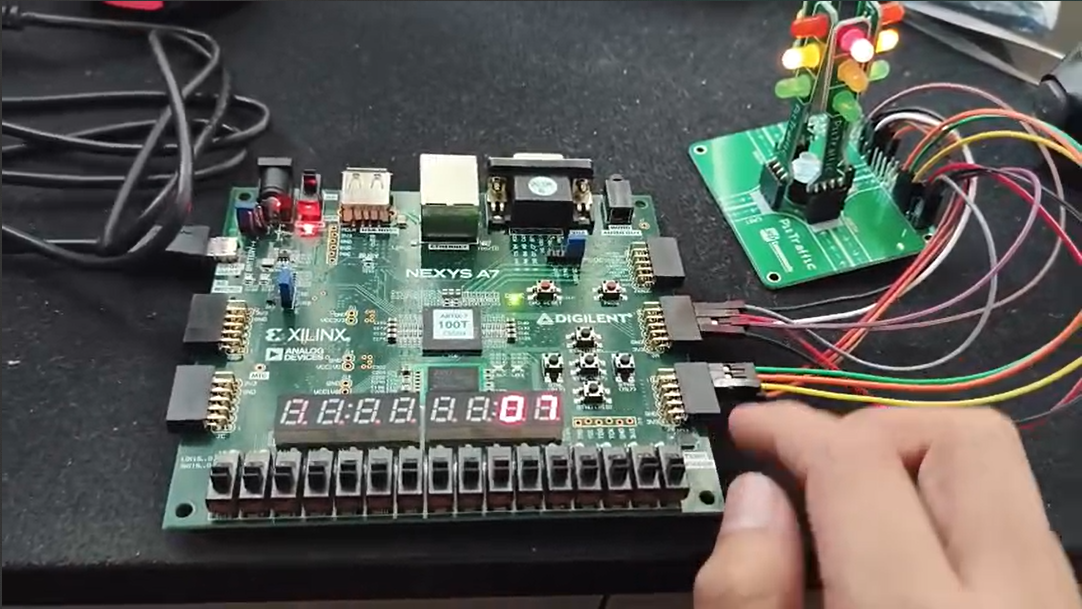
\includegraphics[width=0.65\textwidth]{Resultados/resultado.png}
    \caption{Visualización del semaforo con contador en la Nexys.}
    \label{fig:contador_activo}
\end{figure}




\end{document}
